\documentclass{standalone}
%\usepackage{amsmath,scalerel}
\usepackage{tikz}

\begin{document}
	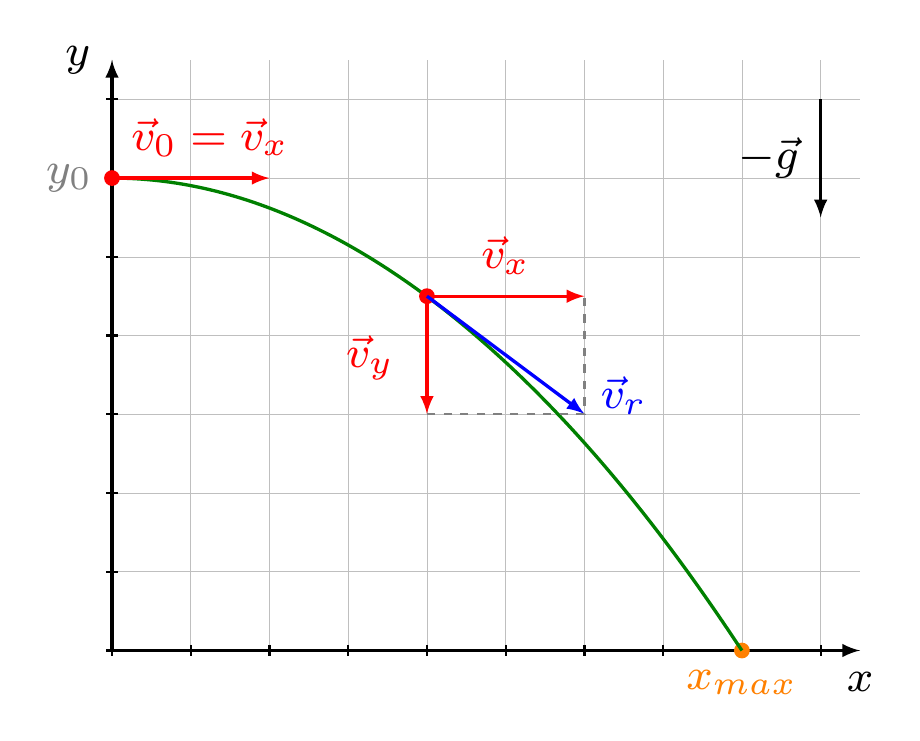
\begin{tikzpicture}
		[
		x=1cm, y=1cm, scale=1.0, font=\footnotesize, >=latex 
		%Voreinstellung für Pfeilspitzen
		]
		
		%Raster im Hintergrund
		\draw[,step=1, gray!50!white, very thin] (0,0) grid (9.5,7.5);
		
		
		%Länge x Achse
		\draw [-latex, very thick] (0,0) -- ++(9.5,0) node[below, scale=2] {$x$};
		
		%Länge y Achse
		\draw [-latex, very thick] (0,0) -- ++(0,7.5) node[left, scale=2] {$y$};
		
		%Zahlen auf y-Achse 
		\foreach \y in {0,1,2,3,4,5,6,7}
		\draw[shift={(0,\y)}, color=black, thick] (2pt,0pt) -- (-2pt,0pt);
		
		%Zahlen auf x-Achse
		\foreach \x in {0,1,2,3,4,5,6,7,8,9}
		\draw[shift={(\x,0)},color=black, thick] (0pt,2pt) -- (0pt,-2pt);
		
		\draw [] (0,6) node[gray, left, scale=2] {$y_{0}$};	
		\draw [] (8,0) node[orange, below, scale=2] {$x_{max}$};	
		\fill [orange] (8,0) circle (0.1);
		% die Parable halt
		\draw[green!50!black, very thick] (0,6) parabola bend (0,6) (8,0);			

		%Vektor v0
		\fill [red] (0,6) circle (0.1);
		\draw[-latex, very thick, red] (0,6) -- ++ (2,0) node [midway, above, red, xshift=7pt, yshift=0pt, scale=2] {$\vec{v}_0=\vec{v}_x$} node (v) {};		
		
		%Vektor v1
		\fill [red] (4,4.5) circle (0.1);
		\draw[-latex, very thick, red] (4,4.5) -- ++ (2,0) node [midway, above, red, xshift=0pt, yshift=0pt, scale=2] {$\vec{v}_x$} node (v) {};
		\draw[-latex, very thick, red] (4,4.5) -- ++ (0,-1.495) node [midway, left, red, xshift=-4pt, yshift=-1pt, scale=2] {$\vec{v}_y$} {};
		\draw[-latex, very thick, blue] (4,4.5) -- ++ (2,-1.495) node [midway, below, blue, xshift=1.5cm, yshift=0pt, scale=2] {$\vec{v}_r$} {};
		\draw [dashed, gray, thick] (4,3)--(6,3)--(6,4.5);
		
		\draw [-latex, very thick] (9,7)--(9,5.5) node [midway, left, xshift=0cm, yshift=0pt, scale=2] {$-\vec{g}$} {};
		
	\end{tikzpicture}

\end{document}

